\scanpage{75}
diagramme qui est déterminé, à isom. unique près, en se donnant un ordre total sur $I$, \inserted{(défini} mod \deleted{\unsure{interversion}} \inserted{transposition} des deux premiers él, et des deux derniers). Pour montrer que deux ordres totaux sur $I$ définissent \deleted{\unsure{une}} des pts de $M^\infty_{0,\nu}$ qui appartiennent à une $=$ composante connexe, il \inserted{suffit de} montrer que deux ordres totaux déduits l'un de l'autre par \inserted{transposition des deux} \unsure{$\varepsilon$|$\in$} $c_i,c_{i+1}$ élts consécutifs sont dans la $=$ composante connexe. Or on le voit en notant qu'on a deux morphismes de générisation \deleted{\unsure{de}} \inserted{dans}
\figure{\begin{tikzpicture}[x=1cm,y=1cm]
\draw (.20,.03)--(.70,.07)--(1.30,.14);
\draw (1.50,.14)--(2.63,.23);
\draw (2.82,.23)--(3.72,.30);
\draw (3.99,.30)--(4.65,.31)--(5.24,.36);
\draw (5.86,.38)--(5.98,.38) (6.18,.40)--(6.40,.44)--(6.54,.43);
\draw (7.42,.47)--(8.54,.60);
\fill (0,0) ellipse (.09 and .045);
\fill (1.30,.14) circle (1.4pt);
\fill (2.63,.23) circle (1.4pt);
\fill (3.72,.30) circle (1.4pt);
\fill (5.24,.36) circle (1.4pt);
\draw[line width=.55pt] (8.95,.56)
 .. controls (8.79,.50) and (8.66,.59) .. (8.72,.69)
 .. controls (8.77,.76) and (8.93,.74) .. (8.93,.66);
\fill (8.82,.70) ellipse (.075 and .045);
\node[above] at (0,.24) {$(c_1,c_2)$};
\node[below] at (0,-.16) {$\unsure{C|c}$};
\node[above] at (1.30,.42) {$c_3$};
\node[above] at (2.63,.62) {$c_{i-1}$};
\node[above] at (3.72,.66) {$(c_i,c_{i+1})$};
\node[above] at (5.24,.73) {$c_{i+2}$};
\node[above] at (8.81,.94) {$c_\nu$};
\end{tikzpicture}}
provient de
\figure{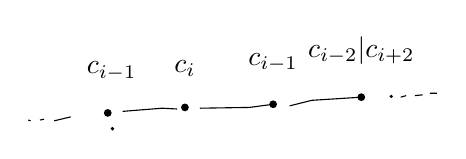
\begin{tikzpicture}[x=1cm,y=1cm]
\draw (-1.01,-.09)--(-.98,-.10) (-.86,-.09)--(-.81,-.08)
 (-.68,-.10)--(-.47,-.05);
\draw (.19,.02)--(.69,.06)--(.88,.05);
\draw (1.17,.06)--(1.80,.07)--(2.10,.11);
\draw (2.31,.09)--(2.59,.16)--(3.22,.20);
\fill (0,0) circle (1.4pt);
\fill (.98,.07) circle (1.4pt);
\fill (2.10,.11) circle (1.4pt);
\fill (3.22,.20) circle (1.4pt);
\fill (.06,-.20) circle (.7pt);
\fill (3.60,.21) circle (.65pt);
\draw (3.72,.20)--(3.79,.22) (3.90,.22)--(4.00,.23)
 (4.09,.25)--(4.18,.25);
\node[above] at (.05,.29) {$c_{i-1}$};
\node[above] at (.98,.34) {$c_i$};
\node[above] at (2.10,.40) {$c_{i-1}$};
\node[above] at (3.22,.49) {$\unsure{c_{i-2}|c_{i+2}}$};
\end{tikzpicture}}
et de
\figure{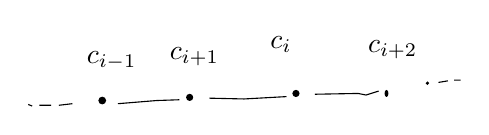
\begin{tikzpicture}[x=1cm,y=1cm]
\draw (-.94,-.05)--(-.89,-.07) (-.80,-.06)--(-.65,-.06)
 (-.55,-.06)--(-.38,-.04);
\draw (.20,-.04)--(.69,0)--(.98,.01);
\draw (1.36,.03)--(1.80,.02)--(2.34,.05);
\draw (2.70,.08)--(3.25,.09)--(3.35,.07)--(3.51,.12);
\fill (0,0) circle (1.4pt);
\fill (1.11,.04) circle (1.3pt);
\fill (2.46,.09) circle (1.3pt);
\fill (3.61,.09) ellipse (.025 and .045);
\fill (4.13,.22) circle (.65pt);
\draw (4.27,.23)--(4.39,.25) (4.47,.26)--(4.55,.26);
\node[above] at (.12,.26) {$c_{i-1}$};
\node[above] at (1.17,.32) {$c_{i+1}$};
\node[above] at (2.27,.48) {$c_i$};
\node[above] at (3.69,.40) {$c_{i+2}$};
\end{tikzpicture}}
en contractant la \deleted{\unsure{seg}} \inserted{arête} qui joint $c_i$ et $\unsure{c_{i-1}|c_{i+1}}$, OK.
\margin{74}
